\section{Усечённая карта и произведение Ли}
\textbf{Вопрос.} Что портит полином степени 3: среднее $\delta$ или само движение?

M3 --- итерация полинома степени 3 того же произведения Ли (это $\mathtt{MAP\_ORDER}$ Bell). Отдельно итерируется само произведение экспонент ($\mathtt{track}$ / $\mathtt{apply\_factor}$). M4 --- точный интегратор. Формула и M2 --- горизонтали, не эталон.

\begin{figure}[H]\centering
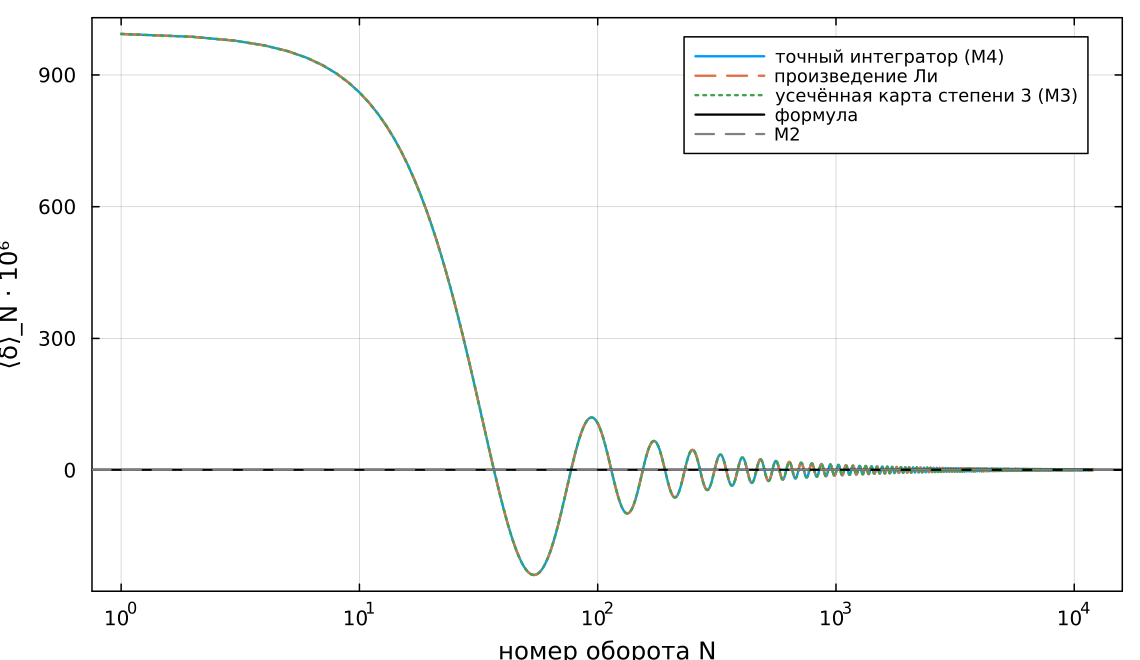
\includegraphics[width=0.92\textwidth]{figs/fig_09_mean.png}
\caption{Скользящее среднее $\delta$. В конце: интегратор $\vMeanExact$, произведение Ли $\vMeanLie$ (разница $\vDiffLieExact$), карта $\vMeanMap$ (разница к интегратору $\vDiffMapExact$).}
\end{figure}

\begin{figure}[H]\centering
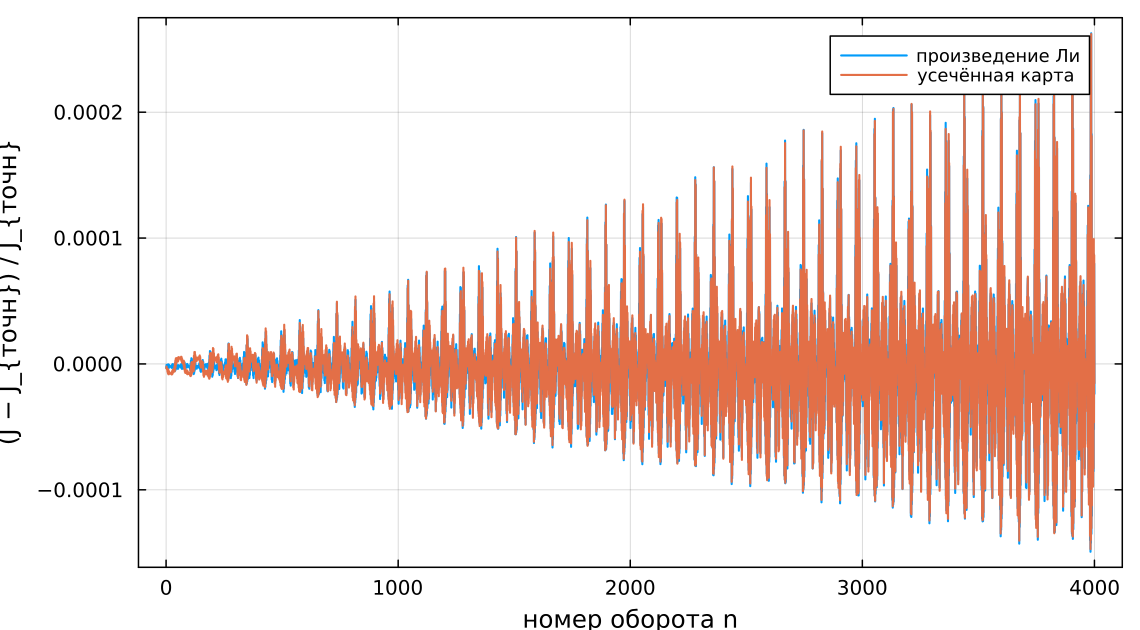
\includegraphics[width=0.92\textwidth]{figs/fig_09_action.png}
\caption{Относительный уход $J_x$ от точного интегратора, $A_x=10$~мм, $N=\vNbact$. Карта: $\vJxRelMap$, произведение Ли: $\vJxRelLie$.}
\end{figure}

\begin{figure}[H]\centering
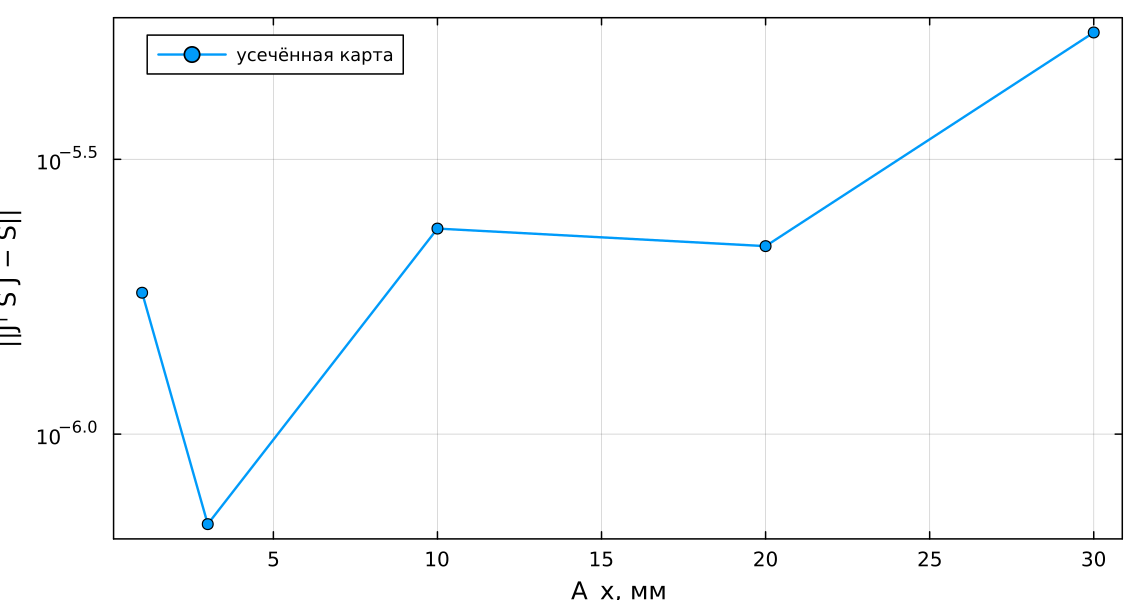
\includegraphics[width=0.92\textwidth]{figs/fig_09_symplectic.png}
\caption{Ошибка симплектичности однооборотного шага усечённой карты: $\vSympSmall$ при 1~мм, $\vSympMap$ при 30~мм. Произведение Ли симплектично по построению (поток генератора).}
\end{figure}

\textbf{Вывод.} Среднее $\delta$ у трёх кривых рядом. На 10~мм за $\vNbact$ оборотов уход действия карты ещё мал ($\vJxRelMap$). Симплектичность карты портится с амплитудой; произведение Ли остаётся симплектичным.
